\chapter{Introduction}
\label{sec:introduction}

This thesis explores and compares the performance of various unsupervised anomaly detection models to automate the identification of faulty soldered pins on \gls{pcb} assemblies. Our goal with this research is to use unsupervised models to eliminate the time-intensive and costly manual labeling process of the dataset to train any supervised learning model. We aim to find a solution with which we can replace the supervised learning model used, by Siemens by using state-of-the-art anomaly detection techniques, to identify defective soldered joints without requiring labeled data. The outcome of this research will be a proposed unsupervised model capable of accurately identifying faults, ultimately improving the production efficiency while reducing pseudo-errors and manual intervention.

Traditionally, inspection of solder joints has been carried out manually or through supervised machine learning models that rely on labeled data. However, the manual labeling process is both time-consuming and expensive. Due to this challenge, unsupervised anomaly detection can become a promising solution. \textbf{Anomalib\cite{Anomalib2024}, a library of state-of-the-art anomaly detection algorithms.} In this thesis, we use Anomalib to explore various unsupervised models, such as PatchCore\cite{roth2022totalrecallindustrialanomaly}, \gls{dfm}\cite{ahuja2019probabilisticmodelingdeepfeatures}, FastFlow\cite{yu2021fastflowunsupervisedanomalydetection} among others. We focus on determining which of these models performs best in detecting defective solder joints, and thereby providing a good alternative to the current supervised methods. %As a result, exploring unsupervised learning techniques which doesn't require labeled data is a good alternative. 

The dataset we use for this study comprises of images of soldered joints on \gls{pcb} boards, provided by siemens. This dataset includes a mixture of images showing both the defect-free called as normal(FC) and defective called as anomalous(NG) soldered joints, with each having dimensions of $512\times512$ pixels. The dataset is divided into training and testing sets, with an 80-20 split for a thorough evaluation of the model. \textbf{Along with that we have set aside 160 images i.e. 80 images per category for the calculation of metric like accuracy etc.} The experiments carried on this dataset includes benchmarking multiple Anomalib models to evaluate their effectiveness in detecting anomalies without the need of labeled data.

Among the models tested, PatchCore emerged to be the best performing model, achieving an accuracy of 91.25\%. Its success can be attributed to its use of locally aware patch features, coreset sampling and the use of memory bank of nominal patch features, allowing for an efficient comparison between new samples and known defect-free examples. The experiments conducted in this thesis provides a comprehensive comparison of unsupervised anomaly detection models. The results suggests that while PatchCore is the most effective unsupervised model for detecting solder joint defects, other models like \gls{dfm}, EfficientAD, and FastFlow also offer unique advantages that could be leveraged depending on specific use-case requirements. incorporating these models into an industrial setting could significantly improve the fault detection process, reducing the dependency on manual inspection, and ultimately lead to more efficient production cycles.

\section{Current Solution at Siemens}
\label{subsec:current solution at siemens}

Before presenting the problem statement, first we give an overview of current supervised solution which is implemented in Siemens. This current solution is described in the figure \ref{fig:solution pipeline}, this solution pipeline begins with first capturing high-resolution images of soldered joints on \gls{pcb} assemblies using an \gls{aoi} machine, which captures images in a batch process and takes under 5 minutes. These images are sent to a server for processing. Then the server runs the \gls{yolo}v8 model, which has been trained on a manually labeled dataset to detect if there is any defect in the image, and classify it either as pass or fail. Due to the supervised nature of this model, it requires a significant amount of labeled data to achieve higher accuracy, and the labeling process of the dataset must be performed by experts with domain specific knowledge. This dependency on labeling not only increases costs but also limits the scalability of the inspection process.

\begin{figure}[ht!]
    \centering
    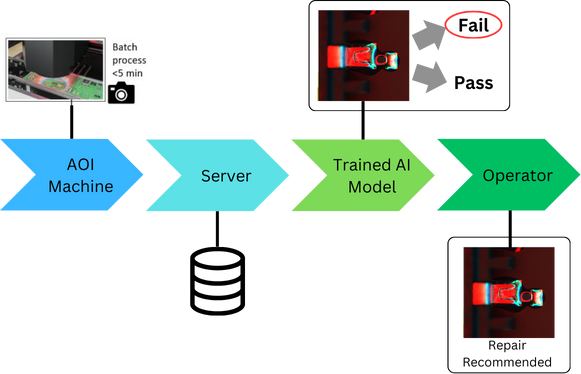
\includegraphics[width=1\linewidth]{Images/Solution_Pipeline.png}
    \caption{Current Siemens solution pipeline}
    \label{fig:solution pipeline}
\end{figure}

The current solution also involves human inspectors who verify the model's recommendations and make final decisions regarding repairs. The operator is responsible for verifying the model's prediction and make the final decision on whether a repair is needed or not. This manual intervention, while still necessary to ensure product quality, adds a layer of complexity and delay to the inspection process. As production demands increases, the dependence on human inspectors can become a bottleneck, preventing the the desired levels of efficiency and throughput. Moreover, the manual nature of this process makes it difficult to achieve consistent inspection quality, as human inspectors may vary in their judgment and expertise.

Given these challenges, there is a clear need for an alternative approach that can address the limitations associated with supervised learning. The unsupervised models explored in this thesis offer a promising solution by eliminating the need for labeled data and providing a more flexible, scalable approach to defect detection. By integrating an unsupervised anomaly detection model into the existing pipeline instead of baseline \gls{yolo} model, the time and cost associated with labeling could be significantly reduced. 

\section{Thesis Objective}

The objective of this thesis is to develop a trained unsupervised anomaly detection model for identification of faulty soldered pins in \gls{pcb} assemblies. This approach aims to reduce the dependency on manual labeling processes while maintaining high accuracy, thereby improving the scalability of the visual inspection process in electronics manufacturing. Specifically, this research seeks to:

\begin{enumerate}
    \item Evaluate the feasibility of using unsupervised anomaly detection models to identify defects in solder joints without requiring labeled datasets.

    \item Benchmark various models from the Anomalib library, which are PatchCore, \gls{dfm}, \gls{dfkde}, EfficientAD, FastFlow, to assess their performance in anomaly detection.

    \item Optimize model's performance through hyperparameter tuning and evaluate the models based on metrics like accuracy, precision, recall, F1-score.
\end{enumerate}

%\section{Thesis Outline}
%This thesis comprises of three main chapters: Theoretical Background, Methodology, and Results \& Discussion.

